\begin{minipage}[c]{\textwidth}
\advance\leftskip-2.5cm
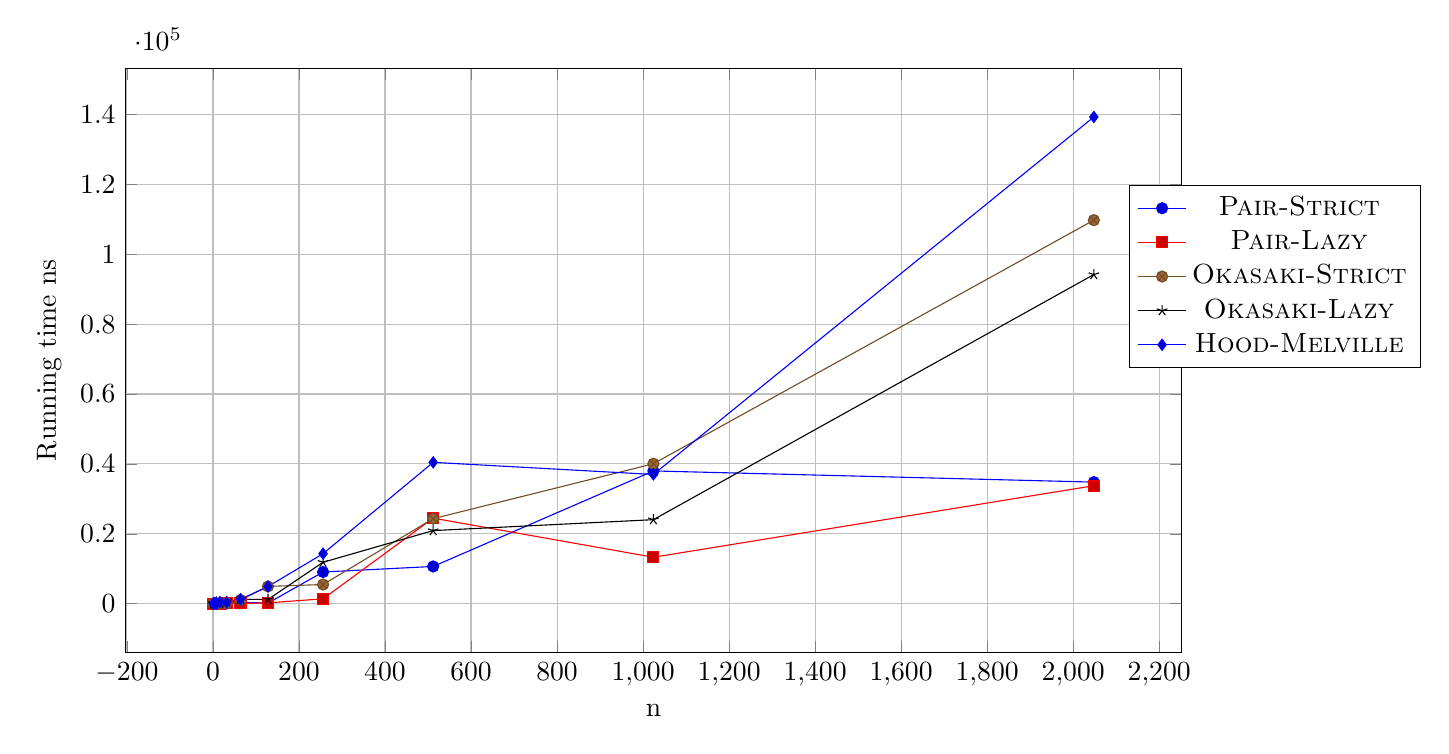
\begin{tikzpicture}
        \begin{axis}[
            xlabel = n,
            ylabel = Running time ns,
            height=9cm,
            width=15cm,
            grid=major,
            legend style={
            at={(0.95,0.8)},
            anchor=north west}]            
            legend pos=center west
    	]
    		
  
                \addplot coordinates {
(1,1)
(2,30)
(4,89)
(8,75)
(16,68)
(32,75)
(64,428)
(128,175)
(256,9076)
(512,10663)
(1024,37992)
(2048,34794)

    	};
        
    	\addlegendentry{\textsc{Pair-Strict}}

        \addplot coordinates {
(1,3)
(2,3)
(4,35)
(8,7)
(16,23)
(32,234)
(64,90)
(128,256)
(256,1398)
(512,24487)
(1024,13297)
(2048,33765)

    	};
        
    	\addlegendentry{\textsc{Pair-Lazy}}

        \addplot coordinates {
(1,13)
(2,3)
(4,56)
(8,46)
(16,47)
(32,112)
(64,1057)
(128,4952)
(256,5494)
(512,24340)
(1024,40046)
(2048,109740)

    	};
        
    	\addlegendentry{\textsc{Okasaki-Strict}}

        \addplot coordinates {
(1,2)
(2,4)
(4,8)
(8,548)
(16,31)
(32,670)
(64,1256)
(128,1223)
(256,11864)
(512,20923)
(1024,24049)
(2048,94180)

    	};
        
    	\addlegendentry{\textsc{Okasaki-Lazy}}

        \addplot coordinates {
(1,3)
(2,26)
(4,136)
(8,30)
(16,455)
(32,388)
(64,1290)
(128,4921)
(256,14323)
(512,40448)
(1024,36979)
(2048,139265)

    	};

    	\addlegendentry{\textsc{Hood-Melville}}

        \end{axis}

    \end{tikzpicture}
    \captionof{figure}{Time of performing multiple inserts and deletes on the same queue}
    \label{fig:sample_figure}
\end{minipage}
